\chapter{Second Prototype Design and Evaluation}
To observe TDT, we compared 
Case 1: \verb|P1_1| and \verb|P1_2| 
Case 2: \verb|P2_1| and \verb|P2_2| (When the interface design has been improved with heuristic evaluation, and the learning content were larger) 

To observe the heuristic guideline, we compared  
Case 3: \verb|P1_1| and \verb|P2_1| 
Case 4: \verb|P1_2| and \verb|P2_2| 

To observe the completed guideline (both TDT and heuristic), we compared 
Case 5: \verb|P1_1| and \verb|P2_2| 
Note: The learning content of \verb|P2_2| were larger

Note: 
\begin{enumerate}
\item Second iteration: The P2 designs (both \verb|P2_1| and \verb|P2_1|) had larger learning content i.e. two learning topics compare to the P1 design (both \verb|P1_1| and \verb|P1_2|) which had one learning content

\item Second iteration: The \verb|P2_2| design had two compulsory assignments, two quiz games.
\end{enumerate} 

\textbf{Result Case 1} 
\begin{figure}[!hbt]\centering
    \begin{subfigure}{0.7\textwidth}
 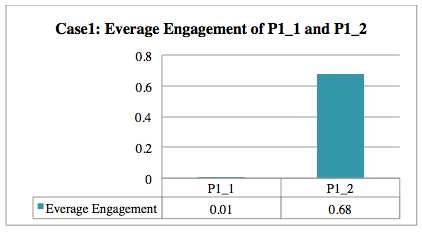
\includegraphics[width=\textwidth]{case1a}
 \caption{Case 1 average engagement}
    \end{subfigure}\hspace{0.1\textwidth}
    \begin{subfigure}{1.0\textwidth}
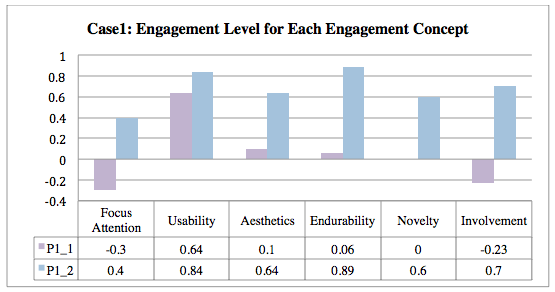
\includegraphics[width=\textwidth]{case1b}
  \caption{Case 1 each engagement concept}
    \end{subfigure}
    \caption{Comparison of engagement  \detokenize{P1_1} and \detokenize{P1_2}}
\end{figure}

The application \verb|P1_2| that followed TDT guideline could engage the participants better (33.5\%) than the application that had the same interface design but did not provide media and functions guide by TDT \verb|P1_1| despite the chat function was crashed and needed a reset if the function had been used. Figure 6.1 presents the comparison of the two prototype designs. 
 
%%%%%%%%%%%%%%%%%%%%%%%%%%%%%%%%%%%%%

\textbf{Result Case 2} 
\begin{figure}[!hbt]\centering
    \begin{subfigure}{0.7\textwidth}
 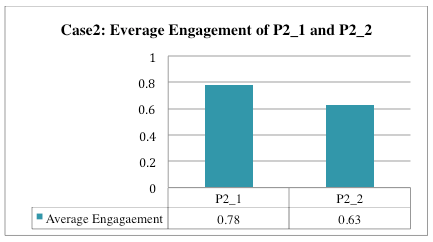
\includegraphics[width=\textwidth]{case2a}
 \caption{Case 2 average engagement}
    \end{subfigure}\hspace{0.1\textwidth}
    \begin{subfigure}{1.0\textwidth}
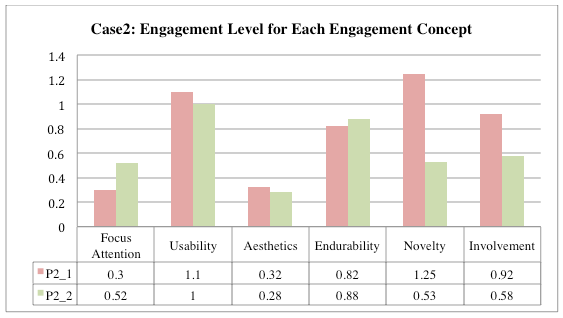
\includegraphics[width=\textwidth]{case2b}
  \caption{Case 2 each engagement concept}
    \end{subfigure}
    \caption{Comparison of engagement  \detokenize{P2_1} and \detokenize{P2_2}}
\end{figure}

We changed learning topic as well as increased the learning content. The interface design also has been improved with heuristic guideline. The chat function has been fixed and worked properly. Participants could use the application smoothly without any reset needed. 

*Results did not repeat the first iteration* 
The application \verb|P2_2| that followed TDT guideline did not engage the participants better than the application that had the same interface design but did not provide media and functions guide by TDT \verb|P2_1| anymore. In fact, the engagement levels of both applications were almost the same. \verb|P1_2| design could engage the participant better only 7.5\%. 

Highlight on "novelty" and "involvement" that the participants gave significant different response.

%%%%%%%%%%%%%%%%%%%%%%%%%%%%%%%%%%%%% 

\textbf{Result Case 3} 
\begin{figure}[!hbt]\centering
    \begin{subfigure}{0.7\textwidth}
 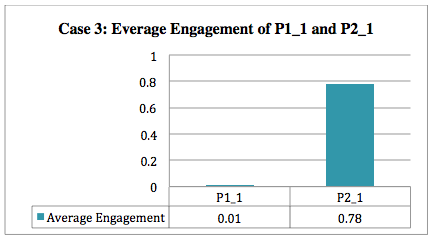
\includegraphics[width=\textwidth]{case3a}
 \caption{Case 3 average engagement}
    \end{subfigure}\hspace{0.1\textwidth}
    \begin{subfigure}{1.0\textwidth}
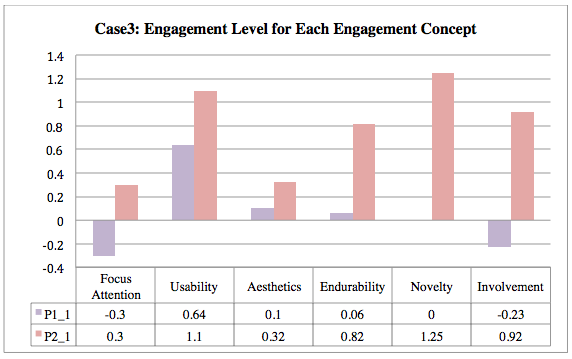
\includegraphics[width=\textwidth]{case3b}
  \caption{Case 3 each engagement concept}
    \end{subfigure}
    \caption{Comparison of engagement  \detokenize{P1_1} and \detokenize{P2_1}}
\end{figure}

Despite \verb|P2_1| had lager learning content and participants were required to learn more and spent more time on the application, they engaged better with \verb|P2_1| compare to \verb|P1_1| (38.5)\% 

Highlight on "Novelty" and "Involvement" 

%%%%%%%%%%%%%%%%%%%%%%%%%%%%%%%%%%%%

\textbf{Result Case 4} 
\begin{figure}[!hbt]\centering
    \begin{subfigure}{0.7\textwidth}
 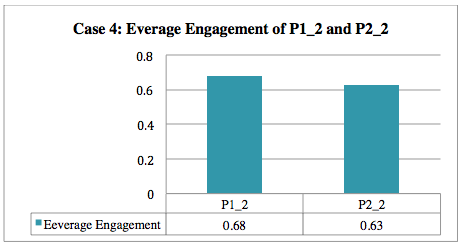
\includegraphics[width=\textwidth]{case4a}
 \caption{Case 4 average engagement}
    \end{subfigure}\hspace{0.1\textwidth}
    \begin{subfigure}{1.0\textwidth}
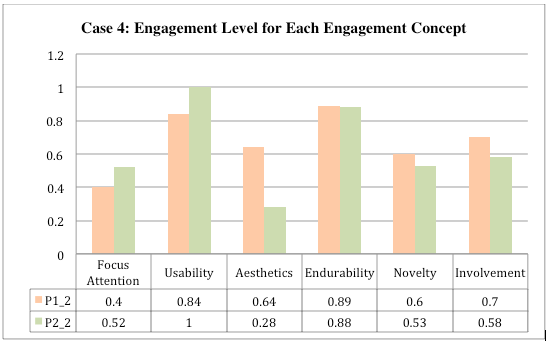
\includegraphics[width=\textwidth]{case4b}
  \caption{Case 4 each engagement concept}
    \end{subfigure}
    \caption{Comparison of engagement  \detokenize{P1_2} and \detokenize{P2_2}}
\end{figure}

The average is pretty much the same \verb|P1_2| engaged better by only 2.5\% 
Only Aesthetics that gave significant different. 

%%%%%%%%%%%%%%%%%%%%%%%%%%%%%%%%%%%%%%

\textbf{Result Case 5} 
\begin{figure}[!hbt]\centering
    \begin{subfigure}{0.7\textwidth}
 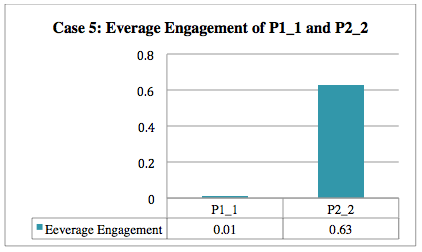
\includegraphics[width=\textwidth]{case5a}
 \caption{Case 5 average engagement}
    \end{subfigure}\hspace{0.1\textwidth}
    \begin{subfigure}{1.0\textwidth}
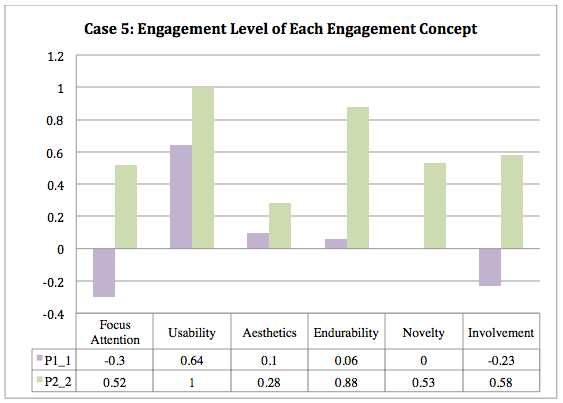
\includegraphics[width=\textwidth]{case5b}
  \caption{Case 5 each engagement concept}
    \end{subfigure}
    \caption{Comparison of engagement  \detokenize{P1_1} and \detokenize{P2_2}}
\end{figure}

Despite the \verb|P2_2| (design that follow the completed guideline including TDT and heuristic evaluation) had lager learning content; it engaged the participant 31\% better than the \verb|P1_1| (design that did not follow neither TDT or heuristic evaluation). 

%%%%%%%%%%%%%%%%%%%%%%%%%%%%%%%%%%%%%

\section{Analysis}
\begin{enumerate}

\item The heuristic evaluation design guidelines had helped the participants to engage with their learning especially the design that does not provide additional media or functions (e.g., games, assignment, and chat). 
*They depended solely on the interface guideline*
When the learning content gets larger, it gets harder to design all the additional media into a small screen of the smart phone. The provided function also required much more effort from the participants especially the compulsory assignments which one of them was a pretty long case study and required an analysis skill to answer the questions. It might be the cause of the decrease of the engagement level. However, the engagement of the design that followed the heuristic evaluation still acceptable. 

\item The TDT guideline had significantly helped to engage the participants that had a weak interface design. For, the application that have already had a good interface design, the additional media such as recorded voice and video and the provided functions such as chat, learning game, and assignment did not help with engagement. Nevertheless, all those media and function might help to improve the understanding and learning quality. 

\item If the application designed followed both TDT and heuristic evaluation guidelines, it improved the engagement level. Based on the previous analysis, the heuristic might played a significant role in increasing the engagement level and TDT might not help much with the engagement. However, the additional media guided by TDT could help the participant who needed extra help, and the functions such as quiz game and assignment would help to practice what they have learnt and the assignment would also could be used by the instructors to check and evaluate the learner progress. 

\end{enumerate} 


 








































